% Dissertação escrita em latex, utilizando a ferramenta abntex, para obtenção do Bachareu em Ciencia da Computação
% pela Universidade Federal Fluminense.
% Autor: Murilo Brugger Stockinger
% Data: 02/11/2017

\documentclass[ruledheader]{abnt_UFF}

%---pacotes para hiphenizacao e acentuacao em portugues
\usepackage[portuguese]{babel}
\usepackage{lmodern}			% Usa a fonte Latin Modern			
\usepackage[T1]{fontenc}		% Selecao de codigos de fonte.
\usepackage[utf8]{inputenc}		% Codificacao do documento (conversão automática dos acentos)
\usepackage[pdftex]{color,graphicx}

%--- pacote para figuras
\usepackage{epsf}
\usepackage[dvips]{epsfig,graphicx}
\usepackage{subfigure}

%--- pacote de simbolos
\usepackage{latexsym}
\usepackage{textcomp}

%--- simbolos matematicos
\usepackage{amsmath}
\usepackage{amssymb}

%--- pacote para gerar pseudo-codigo
\usepackage{algorithm}
\usepackage{algorithmic}
\usepackage{float}

%--- outros pacotes
\usepackage{url}
\usepackage{longtable}
\usepackage{lscape}
\usepackage{booktabs}
%\usepackage{hyperref}%
%Tabela Colorida
\usepackage{colortbl}

\usepackage{tabularx,lipsum,environ,amsmath,amssymb}
\usepackage{diagbox}
\usepackage{amsthm}
\usepackage{svg}
\usepackage{mathtools}



\usepackage{multicol}
\usepackage{multirow}
\usepackage{rotating}

\newcommand{\cclass}[1]{\mathcal{#1}}

\renewcommand{\P}{\textit{P}}
\newcommand{\NPc}{\textit{NPc}}


\renewcommand{\algorithmicend}{\textbf{Fim}}
\renewcommand{\algorithmicif}{\textbf{Se}}
\renewcommand{\algorithmicthen}{\textbf{então}}
\renewcommand{\algorithmicelse}{\textbf{senão}}
\renewcommand{\algorithmicendif}{\textbf{Fim-se}}
\renewcommand{\algorithmicfor}{\textbf{Para}}
\renewcommand{\algorithmicforall}{\textbf{Para todos}}
\renewcommand{\algorithmicdo}{\textbf{faça}}
\renewcommand{\algorithmicendfor}{\textbf{Fim-para}}
\renewcommand{\algorithmicwhile}{\textbf{Enquanto}}
\renewcommand{\algorithmicendwhile}{\textbf{Fim-enquanto}}
\renewcommand{\algorithmicloop}{\textbf{Laço}}
\renewcommand{\algorithmicendloop}{\textbf{Fim-laço}}
\renewcommand{\algorithmicrepeat}{\textbf{Repetir}}
\renewcommand{\algorithmicuntil}{\textbf{até que}}
\renewcommand{\algorithmictrue}{\textbf{Verdadeiro}}
\renewcommand{\algorithmicfalse}{\textbf{Falso}}
\renewcommand{\algorithmicreturn}{\textbf{Retorne}}

\floatname{algorithm}{Algoritmo}
\floatname{table}{Tabela}


\hyphenation{
a-de-qua-da-men-te 
di-men-sio-na-men-to
se-me-lhan-te
}

%---------usando tipo de fonte padrao
\renewcommand{\ABNTchapterfont}{\bfseries\fontfamily{cmr}\fontseries{b}\selectfont}
\renewcommand{\ABNTsectionfont}{\bfseries\fontfamily{cmr}}
\newtheorem{definition}{Definição}
\newtheorem{teorema}{Teorema}
\newtheorem{corolario}{Corolário}
\graphicspath{{../figuras/}}
\newtheorem{axiom}{Axioma}


\newcommand{\Mod}[1]{\ (\mathrm{mod}\ #1)}

% --- -----------------------------------------------------------------
% --- Documento Principal.
% --- -----------------------------------------------------------------
% \usepackage[pdftex]{hyperref}
% \hypersetup{colorlinks, sitecolor=black, pdftex}
\begin{document}

% --- -----------------------------------------------------------------
% --- Titulo, abstract, dedicatorias e agradecimentos.
% --- Indice geral, lista de figuras e tabelas.
% --- -----------------------------------------------------------------
% --- -----------------------------------------------------------------
% --- Elementos usados na Capa e na Folha de Rosto.
% --- EXPRESS�ES ENTRE <> DEVER�O SER COMPLETADAS COM A INFORMA��O ESPEC�FICA DO TRABALHO
% --- E OS S�MBOLOS <> DEVEM SER RETIRADOS 
% --- -----------------------------------------------------------------
\autor{MATHEUS SOUZA D'ANDREA ALVES} % deve ser escrito em maiusculo

\titulo{COLORAÇÃO DE $GRAFOS(r,\ell)$}
\instituicao{UNIVERSIDADE FEDERAL FLUMINENSE}

\orientador{Dr. Uéverton dos Santos Souza }

\local{Niterói}

\data{2018} % ano da defesa

\comentario{Trabalho de Conclusão de Curso apresentado à Universidade Federal Fluminense como requisito parcial para a obtenção do Grau
de Bacharel em Ciência da Computação.}


% --- -----------------------------------------------------------------
% --- Capa. (Capa externa, aquela com as letrinhas douradas)(Obrigatorio)
% --- ----------------------------------------------------------------
\capa

% --- -----------------------------------------------------------------
% --- Folha de rosto. (Obrigatorio)
% --- ----------------------------------------------------------------
\folhaderosto

\begin{center}
    %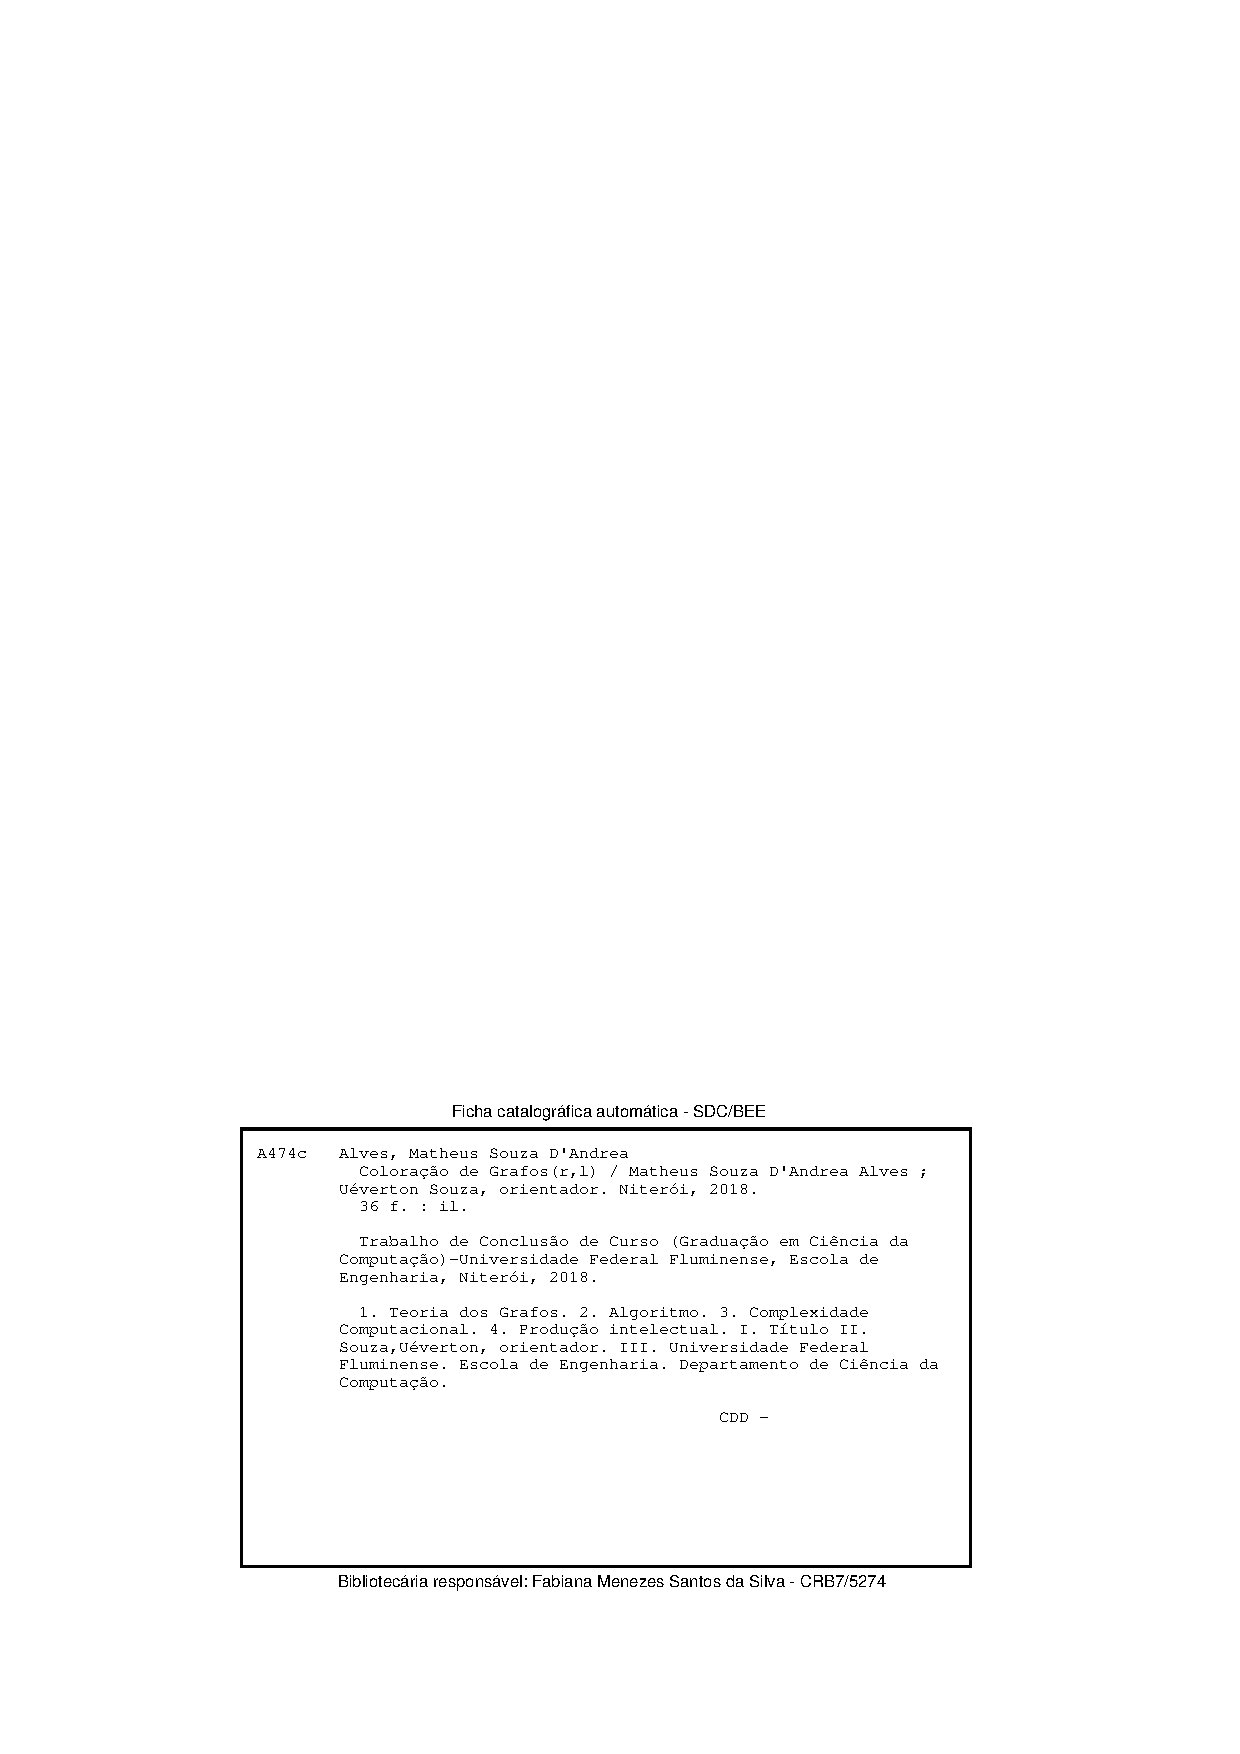
\includegraphics[scale=0.8]{ficha.pdf}    
\end{center}


\pagestyle{ruledheader}
\setcounter{page}{1}
\pagenumbering{roman}

% --- -----------------------------------------------------------------
% --- Termo de aprovacao. (Obrigatorio)
% --- ----------------------------------------------------------------
\cleardoublepage
\thispagestyle{empty}

\vspace{-60mm}

\begin{center}
   {\large MATHEUS SOUZA D'ANDREA ALVES}\\
   \vspace{7mm}
	Coloração de $Grafos(r,\ell)$\\
  \vspace{10mm}
\end{center}

\noindent
\begin{flushright}
\begin{minipage}[t]{8cm}

Trabalho de Conclusão de Curso apresentado à Universidade Federal Fluminense como requisito parcial para a obtenção do Grau
de Bacharel em Ciência da Computação.

\end{minipage}
\end{flushright}
\vspace{1.0 cm}
\noindent
Aprovada em xx/xx/2018. \\ 
\begin{flushright}
   %\includegraphics[scale=0.12]{imagem/nomes.png}
\end{flushright}
  %\parbox{11cm}
  %{
 % \begin{center}
  %BANCA EXAMINADORA \\
%  \vspace{4mm}
%  \rule{11cm}{.1mm} \\
%    Prof$^{\underline{a}}$. Isabel Cristina Mello Rosseti - Orientador, UFF (Presidente)\\
%    \vspace{4mm}
%  \rule{11cm}{.1mm} \\
%    Prof. Marcos Antonio Guerine Ribeiro - Co-orientador, IFRJ\\
%    \vspace{4mm}
%  \rule{11cm}{.1mm} \\
%    Prof. Yuri Abitbol - Avaliador, UFF\\
%    \vspace{4mm}
%   \rule{11cm}{.1mm} \\
%    Prof$^{\underline{a}}$. Simone de Lima Martins - Avaliadora, UFF\\
%    \vspace{4mm}
%  \end{center}
%  }
\begin{center}
  \vspace{6mm}
  Niterói \\
  \vspace{6mm}
  2018
\end{center}

% --- -----------------------------------------------------------------
% --- Dedicatoria.(Opcional)
% --- -----------------------------------------------------------------
%\cleardoublepage
%\thispagestyle{empty}
%\vspace*{200mm}

%\begin{flushright}
%{\em 
%Dedicatoria
%}
%\end{flushright}
%\newpage


% --- -----------------------------------------------------------------
% --- Agradecimentos.(Opcional)
% --- -----------------------------------------------------------------
%\pretextualchapter{Agradecimentos}
%\hspace{5mm}
%Agradecimento

% --- -----------------------------------------------------------------
% --- Resumo em portugues.(Obrigatorio)
% --- -----------------------------------------------------------------
\begin{resumo}
	
Um problema clássico na literatura é o problema de coloração própria de um grafo, isto é, encontrar uma q-coloração para um grafo G tal que todo vértice $v \in V(G)$ não possua nenhum vizinho da mesma cor e q seja mínimo. Esse problema é conhecido ser NP-Difícil para grafos gerais. O trabalho a seguir tem como proposta desvendar e catalogar a complexidade clássica e parametrizada de tal problema para a classe de Grafos$(r,\ell)$, i.e. grafos particionáveis em r conjuntos independentes e l cliques; Identificando as características que tornam o problema difícil e a relação do problema de coloração com outros problemas, quando abordado pela perspectiva parametrizada.

{\hspace{-8mm} \bf{Palavras-chave}}: Complexidade parametrizada. Grafos$(r,\ell)$. Partição de grafos. Coloração de Grafos

\end{resumo}

% --- -----------------------------------------------------------------
% --- Resumo em lingua estrangeira.(Obrigatorio)
% --- -----------------------------------------------------------------
\begin{abstract}

A classical problem in the literature is the problem of proper coloring a graph, i.e. to find a q-coloring for a graph G such that every vertex $ v \in V (G) $ does not have any neighbor of the same color and q is the smallest possible number, a problem known to be NP-Hard for a general graphs. The following work attempts to uncover and catalog the parametrized complexity of such problem for the class of graphs$(r, \ell)$, i.e. partitionable graphs in r independent sets and l cliques; Identifying the characteristics that make the problem hard and the relation of the stated problem to other problems when approached by the parameterized perspective.

{\hspace{-8mm} \bf{Keywords}}: Parametrized Complexity. Graph$(r,\ell)$. Graph Partitioning. Graph Coloring.

\end{abstract}

% --- -----------------------------------------------------------------
% --- Sumario.(Obrigatorio)
% --- -----------------------------------------------------------------
\pagestyle{ruledheader}
\listoffigures
\listoftables
\tableofcontents



% --- -----------------------------------------------------------------
% --- Insercao dos capitulos.
% --- -----------------------------------------------------------------
%\pagestyle{ruledheader}
%\setcounter{page}{1}
%\pagenumbering{arabic}

\chapter{Introdução} \label{cap:intro}

\section{Estruturas básicas}

\subsection{Grafos}
\subsection{Conjunto independente}
\subsection{Clique}
\subsection{Grafos$(r,\ell)$}
\subsection{Bipartição}
\begin{definition}
	Um Grafo dito Grafo$(r,\ell)$ ou abreviadamente $G(r,\ell)$ é qualquer grafo pertencente á classe dos grafos que podem ser particionados em r conjuntos independentes e l cliques.
\end{definition}

\section{Problemas mencionados}

\subsection{Coloração mínima de Grafos}
\begin{definition}
	Entrada: um Grafo $G$ e um inteiro $k$\\
	Questão: Cada vértice pertencente à $G$ pode ser colorido com uma entre $k$ cores
	de tal forma que dado quaisquer dois vértices adjacentes eles tenham cores distintas e $k$ seja o mínimo de cores possível?
\end{definition}

\subsection{Lista coloração de Grafos}
\begin{definition}
  Entrada: Uma paleta de cores $P$ e um Grafo $G$ onde todo $v \in V(G)$ pode ser colorido com um subconjunto $P(v) \subset P$\\
  Questão: É possível escolher uma cor dentro das de $P(v)$ para todo vértice $v$ de forma que dado quaisquer dois vértices adjacentes eles tenham cores distintas?
\end{definition}

\subsection{Clique multicolorida}
\begin{definition}
 Entrada: Um Grafo $G$ com uma k-coloração própria\\
 Questão: Existe em $G$ uma clique que contenha todas as k cores?
\end{definition}

\subsection{PreColoring extension}
\begin{definition}
 Entrada: Um grafo $G$ onde alguns vértices já possuem uma coloração definida com cores escolhidas dentre $k$ possíveis cores.
 Questão: É possível extender a coloração já existente para todo o grafo sem que dois vértices adjacentes possuam a mesma cor? 
\end{definition}

\subsection{Satisfabilidade Ponderada em Circuitos de Entrelaçamento $t$ e Profundidade $h$ \emph{WCS(t,h)}}
\begin{definition}
 Entrada um circuito de decisão $C$ de entrelaçamento $t$ e profundidade $h$\\
 Questão: $C$ possui uma atribuição satisfatível?
\end{definition}

\section{Complexidade clássica}
\subsection{Tratabilidade de tempo polinomial}
Um algoritmo de tempo polinomial é definido como um algoritmo cuja sua função de complexidade de tempo é $\mathcal{O}(p(n))$, para alguma função polinomial $p$, onde $n$ é usado para denotar o tamanho da entrada.

Um problema $\Pi$ pertence à classe $\P$ se e somente se $\Pi$ pode ser solucionado em tempo polinomial por algum algoritmo determinístico.

Um problema $\Pi$ pertence à classe $\textit{Np}$ se e somente se para um dado certificado há um algoritmo polinomial que o verifica sua validade.

\subsection{Reduções}
Dados dois problemas $\Pi$ e $\Pi'$ dizemos que $\Pi \propto \Pi'$ ($\Pi$ se reduz à $\Pi'$ em tempo polinomial) se existe um algoritmo capaz de construir uma instância $J$ de $\Pi'$ a partir de uma instância $I$ de $\Pi$ em tempo polinomial, tal que a partir de uma resposta para $J$ uma resposta para $I$ possa ser construída em tempo polinomial. 

\subsection{NP-Completude}
Um problema $\Pi'$ é dito $NP-Difícil$ se todo problema $\Pi \in NP$ se reduz à $\Pi'$, se $\Pi' \in NP$ então $\Pi'$ é $NP-Completo$.

\section{Complexidade parametrizada}

\subsection{Tratabilidade Parametrizada}
\begin{definition}
Dado um problema $\Pi$ e um conjunto de aspectos de $\Pi$ chamado $S = \{s_1,s_2,s_3,...,s_n\}$ denotamos por $\Pi(S)$ o problema $\Pi$ parametrizado por $S$.
\end{definition}
\begin{definition}
Dado um problema parametrizado $\Pi(S)$ dizemos que o mesmo é FPT(\emph{Fixed parameter tractable} (Tratado por parâmetro fixo)) se existe um algoritmo capaz de resolver $\Pi$ em $\mathcal{O}(f(S)\times n^c)$ onde $f(S)$ é uma função arbritária e $c$ uma função $\mathcal{O}(1)$.
\end{definition}

\subsection{Intratabilidade Parametrizada}
Esta seção irá sumarizar as definições de $W-Hierarquia$ estabelecida por Downey e Fellows, para tanto observe as seguintes definições.
\begin{definition}
 Sejam $\Pi(k)$ e $\Pi'(k')$ onde $k' \leq g(k)$. Chamamos de FPT-redução de $\Pi(k)$ para $\Pi'(k')$ é uma transformação $R$ quando:
 \begin{itemize}
   \item $\forall x, x \in \Pi(k) \iff R(k) \in \Pi'(k')$
   \item $R$ é computável por um FPT-Algoritmo, com relação a $k$
 \end{itemize}
\end{definition}

\begin{definition}
 Um problema parametrizado $\Pi(k)$ pertence a classe $W[t]$ se e somente se existe uma FPT-Redução de tal problema para $WCS(t,h)$ para algum $h$ constante. Logo devido a transitividade de FPT-Redução, se existe uma FPT-Redução de qualquer problema $\Pi'(k')$ para $\Pi(k)$ então $\Pi(k) \in W[t]$
\end{definition}

\chapter{Análise clássica para coloração em Grafos$(r,\ell)$}

\section{Exploração do problema de coloração mínima em Grafos$(r,\ell)$}
O problema de coloração aplicado a Grafos$(r,\ell)$ é de fácil solução para algumas especificações,
por exemplo um Grafo vazio, que é um Grafo(0,0) pode ser colorido com 0 cores, um Grafo disperso i.e um Grafo(1,0) é colorível com apenas uma cor, já que não existem arestas nesse grafo.

Já um Grafo completo, ou seja um Grafo(0,1), é colorível com K cores onde K é a quantidade de vértices nesse grafo completo, em um Grafo split que é um Grafo(1,1) essa regra se repete, já que cada vértice do conjunto independete pode ser colorível com alguma cor já presente na clique.

%primeira tabela de dicotomia
\begin{table}[!htb]
	\center
	\begin{tabular}{l|*{7}c}
		\toprule
		\backslashbox{$r$}{$l$} & 0 & 1 & 2 & 3 & 4 & \ldots & n\\
		\midrule
		0 & \P & \P & ? & ? & ? & \ldots & ?\\
		1 & \P & \P & ? & ? & ? & \ldots & ?\\
		2 & \P & ? & ? & ? & ? & \ldots & ?\\
		3 & ? & ? & ? & ? & ? & \ldots & ?\\
		4 & ? & ? & ? & ? & ? & \ldots & ?\\
		$\vdots$ & $\vdots$ & $\vdots$ & $\vdots$ & $\vdots$ & $\vdots$ & $\ddots$ & ?\\
		n & ? & ? & ? & ? & ? & \ldots & ?\\
		\bottomrule
	\end{tabular}%
	\caption{1ª Dicotomia parcial do problema de coloração em Grafos$(r,\ell)$}
	\label{tab:tabela_part1dictrl}%
\end{table}%

E por fim, Grafos bipartidos são coloridos com 2 cores uma cor para cada conjunto independente.

Sabemos então que coloração é de solução polinomial para grafos completos, dispersos, split e para grafos bipartidos. Assim sendo, temos como ponto de partida para a exploração futura da complexidade de Grafos de cardinalidade superiores a Tabela \ref{tab:tabela_part1dictrl}, a ser preenchida de acordo com os seguintes resultados.

%Teorema que coloração em (3,0) e (0,2) são polinomiais e (4,0) é NPc 
	\begin{teorema}
		Coloração de Grafo(0,2) é Polinomial.
	\end{teorema}
	\begin{proof}
		Um Grafo(0,2) é um grafo separável em 2 cliques, e que todo vértice faz parte de alguma das cliques, logo conhecer a clique máxima é simples e tendo a clique máxima sabemos que o numero mínimo de cores que pode ser usado para colorir o grafo é igual a cardinalidade de tal clique.
	\end{proof}

	\begin{teorema}
		Coloração de Grafo(3,0) é Polinomial.
	\end{teorema}
	\begin{proof}
		Tendo um Grafo G da classe (3,0) como entrada para o problema de coloração sabemos então que o grafo pode ser colorido com 3 cores, resta saber se 3 é o número mínimo de cores que pode ser usado, portanto devemos verificar se G é bipartido (colorível com duas cores) ou um grafo sem arestas (colorível com uma cor), como ambas verificações são polinomiais podemos afirmar que coloração de Grafo(3,0) é resolvível de forma polinomial.
	\end{proof}

	\begin{teorema}
		Coloração de Grafo(4,0) é NP-Completo.
	\end{teorema}
	\begin{proof}
		Sabemos que todo grafo planar é 4-colorível, e que alguns Grafos(4,0) são planares, portanto sabemos que para qualquer Grafo G $\in$ subconjunto de planares de Grafos(4,0), sua quantidade máxima de cores é 4, nos resta saber se 4 também é sua quantidade mínima, porém 3-coloração de planar é NP-Completo logo descobrir a coloração mínima de G é NP-Completo e consequentemente coloração de Grafos(4,0) é NP-Completo
	\end{proof}

É importante notar aqui que, todo $Grafo(r,\ell)$ é simultaneamente um $Grafo(r,\ell+1)$ já que podemos formar uma nova clique trivial utilizando qualquer vértice, e um $Grafo(r+1,\ell)$ já que podemos formar um novo conjunto independente trivial a partir de qualquer vértice, portanto se o problema de coloração é NP-Completo para um $Grafo(r,\ell)$ então ele é NP-Completo para qualquer $Grafo(r+1,\ell)$ ou $Grafo(r,\ell+1)$ .

Esses resultados nos levam à preencher a dicotomia da forma mostrada na Tabela \ref{tab:tabela_part2dictrl}
%Segunda tabela de dicotomia
\begin{table}[htb!]
	\center
	\begin{tabular}{l|*{7}c}
		\toprule
		\backslashbox{$r$}{$l$} & 0 & 1 & 2 & 3 & 4 & \ldots & n\\
		\midrule
		0 & \P & \P & \P & ? & ? & \ldots & ?\\
		1 & \P & \P & ? & ? & ? & \ldots & ?\\
		2 & \P & ? & ? & ? & ? & \ldots & ?\\
		3 & \P & ? & ? & ? & ? & \ldots & ?\\
		4 & \NPc & \NPc & \NPc & \NPc & \NPc & \ldots & \NPc\\
		$\vdots$ & $\vdots$ & $\vdots$ & $\vdots$ & $\vdots$ & $\vdots$ & $\ddots$ & \NPc\\
		n & \NPc & \NPc & \NPc & \NPc & \NPc & \ldots & \NPc\\
		\bottomrule
	\end{tabular}%
	\caption{2ª Dicotomia parcial do problema de coloração em Grafos$(r,\ell)$}
	\label{tab:tabela_part2dictrl}%
\end{table}%

Ainda nos falta mostrar a complexidade para alguns casos de fronteira, que necessitam de uma demonstração mais complexa.
%Demonstrar lista-coloração(r,l)Npc -> coloração(r,l+1)Npc e seus colorários (1,2) & (2,1)

Iremos demonstrar abaixo a complexidade para tais casos utilizando o seguinte teorema. 
\begin{teorema}
\label{theorem:list-coloring}
	Uma solução de lista coloração para um grafo $G(r,\ell)$, implica em uma solução para o problema de coloração de um grafo $H_G(r,\ell+1)$.
\end{teorema}
\begin{proof}
	Para a demonstração é preciso mostrar que
	\begin{itemize}
		\item Se um grafo G$(r,\ell)$ possui uma lista coloração própria então $H_G$ é k-colorível para k do tamanho da paleta $C$ (1)
		\item Se $H_G$ é k-colorível então G possui uma lista coloração própria (2)
	\end{itemize}
	(1):\newline
	
	Usaremos a seguinte construção:\newline
	Considere G um grafo$(r,\ell)$ e que para cada vértice $v \in V(G)$ exista uma lista de cores $S_v$ referente a esse vértice, cada lista contém pelo menos uma cor da paleta $C = \{c_1,c_2,c_3,...,c_k \}$, sendo G uma instância sim para o problema de lista coloração, criemos uma clique K onde cada vértice $k \in V(K)$ representa uma cor presente em $C$. Seja $H_G = G \cup K$ para todo vértice $v \in G$ e todo vértice $u_i \in K$ adicione uma aresta $(u_i,v)$ à $H_G$ se e somente se v não possui a cor $c_i$ em sua lista coloração em G
	
	Podemos então generalizar da seguinte forma, dado um grafo$(r,\ell)$ $G$ onde cada vértice de $G$ possui uma lista de possíveis cores então o grafo $H_G$ obtido pela construção anterior possui uma k-coloração.
	
	Note que a clique K possui exatamente k vértices, consequentemente para colorirmos K precisaremos de k cores, sem perda de generalidade assumimos que $u_1$ será colorido com $c_1$, $u_2$ com $c_2$ e assim por diante.
	
	Por construção uma aresta de $u_i$ só existe para $v_a$ em $H_G$ se e somente se, $v_a$ não possui $c_i$ em sua lista de cores, portanto a coloração atribuída à K não conflita com a com a lista coloração de G, e portanto para todo vértice perntecente a G podemos lhe atribuir a mesma cor que lhe foi atribuída no problema de lista coloração, obtendo uma coloração própria mínima para $H_G$
	
	(2):\newline
	Suponha que o grafo $H_G$ possua uma k-coloração própria, onde k é o número de cores nas listas de G
	
	Seja K a maior clique presente em $H_G$, por construção $H_G$ é colorível com k cores onde k é a cardinalidade de K, observe que a remoção de K não afeta a coloração de $H_G - K$
	
	Como $H_G$ é k-colorível e a clique K possui k vértices todas as cores de tal k-coloração estão presentes em K. Sem perda de generalidade podemos assumir que as cores $c_1,c_2,...,c_k$ estão atribuídas aos vértices $u_1,u_2,...,u_k$ pertencentes à K
	
	Por construção de $H_G$ todo par $(v,u_i)$ onde $v \in H_G - K$ e $u_i \in K$ é não adjacente se e somente se o vértice $v$ não possui $c_i$ em sua lista coloração no grafo $G$
	
	Logo a k-coloração atribuídas aos vértices em $H_G - K$ formam uma coloração para G onde todo vértice em $V(G)$ possui uma cor de sua lista. Portanto G é uma instância sim de lista coloração
\end{proof}
Portanto utilizando o teorema \ref{theorem:list-coloring}, derivamos os seguintes corolários:
\begin{corolario}
	O problema de coloração é NP-Completo para Grafos$(1,2)$.
	\begin{proof}
		A NP-Completude de lista coloração em grafos split i.e. grafos$(1,1)$ é demonstrado por Jensen et al. \cite{jansen1997}.
	\end{proof}
\end{corolario}
\begin{corolario}
	O problema de coloração é NP-Completo em Grafos$(2,1)$.
	\begin{proof}
		A NP-Completude de lista coloração em grafos bipartido é demonstrado por Fellows et al. em \cite{fellows07}.
	\end{proof}
\end{corolario}    
\begin{corolario}
	Se lista coloração é NP-Completo para Grafos(0,2) então Coloração é NP-Completo em Grafos(0,3).
	\begin{proof}
		Para essa demonstração nos basearemos em um resultado obtido por Jensen em \cite{jansen1999}. a demonstração se baseia em realizar uma redução do problema 3-SAT restrito para lista coloração de co-bipartido i.e. Grafo(0,2).
		Suponha o problema 3-SAT com as seguintes restrições:
		\begin{itemize}
			\item cada cláusula $c_i$ contém dois ou três terminais.
			\item cada terminal ou sua negação aparece no máximo em 3 cláusulas
		\end{itemize}
		Construiremos agora uma instância de lista coloração da seguinte forma:\newline
		Para cada terminal $j$ crie seis vértices:
		$a_j^{(1)}$, $a_j^{(2)}$, $a_j^{(3)}$;
		$b_j^{(1)}$, $b_j^{(2)}$, $3_j^{(3)}$. Atribuindo a cada uma lista de cores da seguinte forma:\newline
		$a_j^{(k)}$ <= \{$x_j^{(k)}$, $\overline{x_j}^{(k)}$ \}; $b_j^{(k)}$ <= \{$\overline{x_j}^{(k)}$,$x_j^{((k \Mod{3}) + 1 )}$ \}\newline
		Definimos como A o conjunto de todos os $a_j^{(k)}$ e B o conjunto de todos os $b_j^{(k)}$ e construímos uma clique com os vértices de A e B. Observe que só existem duas maneiras de se colorir este grafo:
		\begin{itemize}
			\item (1)  $f(a_j^{(k)}) = x_j^{(k)} => b_j^{(k)} = \overline{x_j}^{(k)}$
			\item (2)  $f(a_j^{(k)}) = \overline{x_j}^{(k)} => b_j^{(k)} = x_j^{((k \Mod{3}) + 1 )}$
		\end{itemize}
		Agora, para cada cláusula definimos um vértice $c_i$ e sua lista de cores da seguinte forma: para cada literal $j$ ou sua negação $\overline{j}$ presente na cláusula adicionamos à lista de $c_i$ o $x_j^{(k)}$ onde k é o indice de ocorrência do literal ou de sua negação.
		
		Por exemplo, suponha o seguinte 3-SAT:
		
		$(p \lor q \lor r) \land (\neg{p} \lor q \lor r) \land (\neg{p} \lor \neg{r} \lor s)$
		
		suas cláusulas seriam traduzidas para
		\begin{itemize}
			\item $c_1$ com lista: \{$p^1$, $q^1$, $r^1$ \}
			\item $c_2$ com lista: \{$\overline{p}^2$, $q^2$, $r^2$ \}
			\item $c_3$ com lista: \{$\overline{p}^3$, $\overline{r}^3$, $s^1$ \}
		\end{itemize}
		Seja C o conjunto contendo todos os $c_i$ criamos uma clique com $C \cup A$.
		Nosso grafo tem portanto a seguinte configuração(considere $x'$ como $\overline{x}$):
		\begin{figure}[!ht]
			\centering
			\includesvg{3-SAT.svg}
			\caption{Grafo G: Transformaçao de 3-SAT em co-bipartido com foco na cláusula P }
		\end{figure}
		
		Suponha a cláusula p, se p é verdadeiro então $a_p^{(1)},a_p^{(2)},a_p^{(3)}$ será colorido com $p'^1,p'^2,p'^3$, permitindo que a cor $p^x$ possa, e que a cor $p'^x$ não possa ser escolhidas para colorir uma cláusula.
		
		De tal forma, podemos facilmente notar que, expandindo a explicação anterior para os outros terminais uma resposta sim para o problema 3-SAT restrito nos leva a uma solução do problema de lista coloração em co-bipartido por exclusão das cores nas listas disponíveis. Para a volta a existência de uma lista coloração válida para o co-bipartido mostra uma solução para o 3-SAT restrito correspondente simplesmente descobrindo a representação em valor de terminal das cores escolhidas para as cláusulas. 
		
	\end{proof}
\end{corolario}
Portanto podemos agora completar nossa tabela com:
\newpage
\begin{table}[!htb]
	\center
	\begin{tabular}{l|*{7}c}
		\toprule
		\backslashbox{$r$}{$l$} & 0 & 1 & 2 & 3 & 4 & \ldots & n\\
		\midrule
		0 & \P & \P & \P & \NPc & \NPc & \ldots & \NPc\\
		1 & \P & \P & \NPc & \NPc & \NPc & \ldots & \NPc\\
		2 & \P & \NPc & \NPc & \NPc & \NPc & \ldots & \NPc\\
		3 & \P & \NPc & \NPc & \NPc & \NPc & \ldots & \NPc\\
		4 & \NPc & \NPc & \NPc & \NPc & \NPc & \ldots & \NPc\\
		$\vdots$ & $\vdots$ & $\vdots$ & $\vdots$ & $\vdots$ & $\vdots$ & $\ddots$ & \NPc\\
		n & \NPc & \NPc & \NPc & \NPc & \NPc & \ldots & \NPc\\
		\bottomrule
	\end{tabular}%
	\caption{Dicotomia do problema de coloração em Grafos$(r,\ell)$}
	\label{tab:tabela_dictrl}%
\end{table}%

\chapter{Análise parametrizada para coloração em Grafos(2,1)}
Tendo mostrado a complexidade clássica nos é interessante agora que elucidemos quais caractéristicas dos grafos$(r,\ell)$ se mostram propícias a abordagem parametrizada, a cardinalidade de suas partições se mostrou uma interessante característica.
Decidimos abordar a classe (2,1), já que a mesma é a classe onde o problema é NP-Completo com o menor número de partições.

Um Grafo(2,1) é um grafo particionado em 2 conjuntos independentes e 1 clique, portanto ele nos entrega 3 naturais candidatos a parametrização, o tamanho da clique $\ell$, o tamanho do menor conjunto independente $r_1$ e o tamanho do maior conjunto independente $r_2$.

\section{Parametrização pelo tamanho do menor conjunto independente}
Em \cite{fellows07} Fellows (et. al) mostrou que o problema de lista coloração é $W[1]-difícil$ parametrizado pela treewidth através da transformação do problema da clique multicolorida parametrizada pelo tamanho da clique para tal, nos aproveitaremos dessa transformação para mostrar que:
\begin{teorema}
	Coloração em Grafos(2,1) é $W[1]-difícil$ quando parametrizado pelo tamanho do menor conjunto independente.
\end{teorema}
\begin{proof}
	Observe a seguinte transformação.
	
	O problema da clique multicolorida é conhecidamente $W[1]-difícil$\cite{fellows07}.
	
	Portanto suponha tal $G$ proposto ao problema de clique multicolorida, temos como intenção montar um problema de lista coloração em um grafo $G'$ a partir dele, para tanto seguimos os seguintes passos:
	\begin{itemize}
		\item Para cada cor $i$ presente em $G$ cria-se em $G'$ um vértice $v_i$ (os chamaremos de vértices-cor).
		\item Para cada vértice $u$ em $G$ colorido com a cor $i$, adicionamos à lista do vértice-cor $v_i$ em $G'$ uma cor $c_u$ relacionada a esse vértice (as chamaremos de cores-vértice).
		\item Para cada aresta $e(x,y) \notin E(G)$ onde $x,y \in V(G)$ cria-se em $G'$ um vértice $z_e$ adjacente ao vértice-cor $v_i$ onde $i$ representa as cores de $x$ e $y$, a lista coloração de $z_e$ será formada por $c_x$ e $c_y$.
	\end{itemize}
	É notável que a treewidth de $G'$ é dada por $k$, já que a remoção dos vértices-cor leva a um grafo sem arestas. Assim sendo se $G$ possui uma clique multicolorida podemos facilmente colorir $G'$ da seguinte forma:
	
	Ao vértice-cor $v_i$ atribua a cor-vértice $c_u$ onde $u$ é o vértice colorido com a cor $i$ em $G$. Dessa forma todos os vértices $z_e$ possuem ainda uma cor disponível para sua coloração já que ele representa uma não-aresta em $G$. 
	
	Para a volta observe que uma lista coloração válida em $G'$ implica em uma clique multicolorida em $G$, isso se dá pois dois vértices $x,y$ coloridos com cores diferentes em $G$ não aparecem em uma lista de algum $z_e$ em $G'$ se e somente se existe uma aresta $e(x,y) \in E(G)$, portanto as cores-vértices escolhidas para os vértices $v_i$ são uma respectivamente uma clique formadas por tais $i$ em $G$. Mostramos assim que lista coloração parametrizada por treewidth é $W[1]-difícil$.
	
	Sabemos que coloração em Grafos(2,1) é equivalente a lista coloração em um grafo bipartido, portanto nossa tentativa de parametrizar a coloração de (2,1) pelo tamanho do menor conjunto independente é equivalente a parametrizar lista-coloração em bipartidos pelo tamanho do menor conjunto independente, é de pouca dificuldade ver que a treewidth de um grafo bipartido existe em função do menor independente, mostrando assim que coloração em Grafos(2,1) parametrizada pelo tamanho do menor conjunto independente é $W[1]-difícil$. 
	
\end{proof}

\section{Parametrização pelo tamanho do maior independente}

 Sabemos agora que a parametrização pelo menor independente não nos traz um algoritmo FPT, porém ao analisarmos o comportamento do problema quando parametrizado pelo maior independente vemos que a limitação do tamanho de $r2$ também limita $r1$; Tendo tal limitação a utilização de um método força bruta se mostra uma abordagem válida, como mostrado o seguinte teorema.
\begin{teorema}
  Coloração de Grafos(2,1) é FPT quando parametrizado pelo tamanho do maior conjunto independente.
\end{teorema}
\begin{proof}
  Para tal demonstração onde $k$ é o tamanho de $r2$, observe que são necessárias pelo menos $t$ cores, onde $t$ é a cardinalidade da clique para colorir tal grafo, novamente usaremos a estratégia de transformar coloração de (2,1) em lista coloração de bipartido.
  
  Em uma lista coloração de bipartido, se um vértice possui uma lista com mais cores do que o tamanho de sua vizinhança, ele sempre terá disponível uma cor para sua coloração, podemos portanto remover esse vértice do grafo sem alterar sua coloração, ao chegarmos ao ponto onde todo vértice com tal configuração foi removido temos que $t$ está limitado em função de $k$, portanto rodar um algoritmo de força bruta para encontrar a coloração se mostra FPT.     
\end{proof}

\section{Parametrização pelo tamanho da clique}

Para a demonstração da complexidade parametrizada utilizando $k=\#\ell$ nos voltamos novamente para transformação da clique em um Grafo(2,1) em listas coloração do restante bipartido, dessa forma nosso problema parametrizado original se torna um novo problema, lista coloração de bipartido parametrizado pelo tamanho da paleta de cores. 

Mostraremos no entanto que essa parametrização não é proveitosa já que o problema se mostra equivalente à PreColoring Extension com limite de cores, mostrado ser NP-Completo para grafos bipartidos mesmo quando sua paleta é de tamanho 3\cite{kratochvil94}.

\begin{teorema}
	Lista coloração em bipartidos é NP-Completo
\end{teorema}
\label{theorem:list-coloring-bipartide}
\begin{proof}
	Suponha uma instância $P$ do problema PreColoring Extension e $G$ seu grafo de entrada, sabemos que $G$ possui uma paleta $C$ de cores de tamanho definido, e que existem $v \in V(G)$ que já estão coloridos com uma cor $c \in C$, podemos ver tal configuração como um grafo $G'$ onde os vértices $v$ possuem listas contendo apenas $c$, e os demais vértices possuem listas de tamanho $\#C$ contendo todas as cores, nos levando a um problema de lista coloração $Q$ que tem como entrada $G'$.
	
	Uma coloração possível para $G$ implica em uma coloração possível para $G'$, já que nos basta atribuir aos vértices em $G'$ as mesmas cores atribuídas em $G$. De forma análoga, uma lista coloração possível em $G'$ implica em uma coloração possível em $G$.
\end{proof}


Apesar do tamanho da paleta não ter se mostrado uma escolha adequada, ele levanta novos parametros que são interessantes para o problema de lista coloração em bipartidos, observe pois que, sabemos que Precoloring extension é polinomial se todas as listas tem tamanho 1 ou 2 \cite{hujter93}, e NP-Completo se todas tem listas e tamanho 1 à 3 \cite{kratochvil94}, isso levanta duas formas de se abordar o problema, o que acontece quando o número de vértices com listas de tamanho 1 e 2 varia, e o que acontece quando o número de vertices com listas de tamanho 3 varia.

Mostraremos nas próximas seções como se dão tais comportamentos e como eles se relacionam a coloração de Grafos$(r,\ell)$

\section{Parametrizado pela quantidade de vértices vizinhos à clique}
Nos focaremos nessa seção em grafos(2,1) cuja a clique tenha tamanho 3, já mostrada ser o menor tamanho necessário para que o problema de seja NP-Completo mostrado no teorema \ref{theorem:list-coloring-bipartide} e em \cite{kratochvil94}. Portanto um vértice que é vizinho da clique tem necessariamente uma lista contendo uma ou duas cores, já que um vértice não pertencente a clique que tenha lista de tamanho zero deveria fazer parte da clique, em contrapartida um vértice com lista tamanho 3 é um vértice não vizinho a clique. 

Mostraremos que mesmo quando parametrizado pela quantidade de vértices com listas de tamanho um, dois, ou um e dois o problema é Para-Np-completo. Para tanto é necessário encontrar uma instância do problema já parametrizado cuja solução permanece igualmente difícil.

Portanto essa seção será dividida em três casos, um contendo vértices de listas tamanho um, outro contendo vértices com listas de tamanhos dois, e finalmente contendo listas de tamanho um e dois.
\subsection{Apenas vértices com listas tamanho um}
É importante ressaltar que os seguintes teoremas estabelecem a base para a resolução do problema envolvendo os vizinhos da clique. 
\begin{teorema}
 \label{teorema:6-v-np}
  Seis vértices com lista de tamanho um são necessários para que lista coloração em bipartido seja Para-NP-completo. 
\end{teorema}
\begin{proof}
 Sabemos que em nosso problema temos dois conjuntos independentes, $r1$ e $r2$, também é verdade que exceto pelos citados seis vértices todos os outros vértices tem listas de tamanho três, os vértices de $r1$ podem estar ligados arbitrariamente aos vértices de $r2$. 
 
 Observe a disposição da figura \ref{fig:seis-vertices-lista-um}
 
\begin{figure}[H]
		\centering
		\includesvg[scale=0.6]{seis-vertices-lista-um.svg}
		\caption{Uma possível instância formada por 6 vértices com listas tamanho 1. }
		\label{fig:seis-vertices-lista-um}
\end{figure}

Observe como a presença de um vértice com uma lista de tamanho um influencia em sua vizinhança; a existência desse vértice implica na remoção de sua única possível cor das listas de seus vizinhos, a estrutura mostrada na figura \ref{fig:seis-vertices-lista-um} mantém a coloração do restante NP-Completo ao restringir a cor dos vizinhos sem ter o controle da estrutura resultante perdendo portanto o viés parametrizado.

\end{proof}

Interessantemente o problema é de trivial solução quando o número de vértices com listas tamanho um é zero, já que se torna o problema de 3-coloração em bipartidos, mas NP-Completo com 6 vértices, queremos portanto notar qual é o menor número de vértices no qual o problema é NP-Completo, e consequentemente Para-NP-Completo para nossa parametrização.

\begin{teorema}
\label{lemma:1-col-P}
 Lista coloração em bipartido é de solução trival quando há apenas um vértice de lista tamanho um.
\end{teorema}
\begin{proof}
 Sabemos que além do vértice citado todos os outros vértices têm listas de tamanho três dessa forma basta que o conjunto independente no qual tal vértice está inserido seja colorido com a única cor escolhida para o vértice e o conjunto independente sobrante pode ser colorido com qualquer cor.
\end{proof}

\begin{teorema}
 Lista coloração em bipartido é de solução linear quando existem dois vértices de lista tamanho um.
\end{teorema}
\begin{proof}
 Para essa demonstração é necessária a observação em que existem duas possíveis configurações para essa instância:
 \begin{itemize}
   \item Ambos os vértices pertencem ao mesmo conjunto independente.
   \item Os vértices pertencem a conjuntos distintos.
 \end{itemize} 
 No primeiro caso a estratégia usada no lema \ref{lemma:1-col-P} pode ser adaptada para a solução. Para tanto basta colorir tais vértices com suas cores disponíveis e o conjunto independente ao qual pertencem com a cor de algum deles, e o conjunto sobressalente com a cor restante.
 
 No segundo caso, a coloração também é simples. Se tais vértices tem cores distintas basta colorir seus respectivos conjuntos com a mesma cor. Se não, como temos três cores podemos colorir os vértices com a cor 1, um conjunto com a cor 2 e os demais vértices com a cor 3.  
\end{proof}

\begin{teorema}
  Três vértices com lista de tamanho um são suficientes para que lista coloração em bipartido seja NP-completo.
\end{teorema}
\begin{proof}
  Mostraremos aqui como que três vértices são suficientes para que o problema seja NP-Completo, esse resultado se dá pois é possível reproduzir a estrutura do teorema \ref{teorema:6-v-np} utilizando os ditos 3 vértices, para tanto basta que notar o seguinte \emph{gadget}:
  
\begin{figure}[H]
  \begin{subfigure}
    \centering
		\includesvg[scale=0.6]{gadget-1.svg}
  \end{subfigure}
  \begin{subfigure}
    \centering
		\includesvg[scale=0.6]{gadget-2.svg}
  \end{subfigure}
  \begin{subfigure}
    \centering
		\includesvg[scale=0.6]{gadget-3.svg}
  \end{subfigure}
  \caption{Gadget com vértices de lista um reproduzindo vértice de lista um em vértice de lista três}
\end{figure}

Usando tal gadget usando dois vértices com lista um em um vértice com lista três é possível reproduzir um vértice de cor um, sendo assim tendo três vértices de lista um é possível obter seis vértices de lista um e reproduzir a estratégia mostrada no teorema \ref{teorema:6-v-np}, que nos mostra a NP-Completude desse problema.
  
\end{proof}
 Dado os resultados apresentados nessa seção mostramos portanto que o numéro de vértices vizinhos a dois dos três vértices pertencentes a clique não é um parâmetro viável para uma solução FPT.
  
\subsection{Vértices com listas de tamanho dois}
Mostraremos nessa seção que vértices com listas tamanho dois não são suficientes para que um algoritmo FPT seja extraído.

Como já visto o problema é de trivial solução quando todos os vértices tem listas de tamanho três, portanto precisamos ainda encontrar qual número de vértices de tamanho dois onde o problema se torna NP-Completo.

\begin{teorema}
 Seis vértices com listas tamanho 2 são necessários e suficientes para que lista-coloração em bipartido seja NP-Completo.
\end{teorema}
\begin{proof}
 Para mostrarmos que qualquer número de vértices abaixo de 6 é insuficiente, mostraremos que a menos que existam pelo menos 3 vértices com lista tamanho dois em cada conjunto independente, a coloração é simples de ser feita. 
 
 Se um conjunto independete contém apenas dois vértices com listas tamanho dois, podemos afirmar que todos os vértices nesse conjunto compartilham uma cor em suas listas, podendo colorir tal conjunto com essa cor, todos os outros vértices ainda têm pelo menos uma cor disponível para sua coloração podendo ser colorido com ela.
 
 Para completar nossa demonstração basta encontrar uma configuração onde o problema de lista coloração permanece NP-Completo.
 observaremos agora a vizinhança dos vértices com lista dois, iremos isolar as instâncias em alguns casos, separando sem perda de generalidade um vértice.
 \begin{itemize}
   \item Vizinhança de tamanho um.
   Nesse caso podemos notar que independentemente do vértice e seu vizinho eles sempre compartilharão uma cor, colorimos o vértice de $r2$ com tal cor, além disso como conheçemos a vizinhança sabemos que nenhum outro vértice é vizinho deste, podemos então colorir os restantes vértices de $r2$ com a cor remanescente, dessa forma uma das três cores ainda resta e podemos a usar para colorir o restante do $r1$.
   \begin{figure}[H]
     \centering
     \fontsize{6}{10}
     \includesvg[scale=0.5]{1-edge.svg}
     \caption{Demonstração de coloração para vizinhança de tamanho 1.}
   \end{figure}
 \end{itemize}
\end{proof}

\subsection{Vértices com listas de tamanho um e dois}

Para o acontecimento de haver vértices com listas tamanho um e dois, basta notar que podemos pintar aqueles que contém listas de tamanho um, que propagará a remoção de sua cor aos vizinhos, e ao realizar isso iterativamente, acabaremos com um caso em que todos os vértices terão ou listas de tamanho dois ou três, caindo em algm dos casos supracitados.

\section{Parametrizado pela quantidade de vértices não vizinhos a clique}
Como visto na seção anterior, os vértices que não são vizinhos a clique, quando transformados em vértices do problema de lista coloração se transformam em vértices com listas tamanho três, portanto nosso desejo é resolver lista coloração em bipartidos com listas de tamanho um a três parametrizado pela quantidade de vértices com lista de tamanho três, a solução deriva do seguinte teorema.

\begin{teorema}
 Lista coloração em bipartidos com listas de tamanho um a três é FPT quando parametrizado pela quantidade de vértices com lista de tamanho três
\end{teorema}
\begin{proof}
 Dado que temos $k$ vértices com 3 escolhas cada é possível montar um algoritmo de busca em árvore de altura limitada de tamanho $3^k$, e então executar o algoritmo linear proposto em \cite{hujter93} obtendo um algoritmo $\mathcal{O}(3^kn)$
 
\end{proof}

\chapter{Conclusão} \label{cap:conclusao}
Apresentamos aqui o desenvolvimento e especificações da dificuldade do problema de coloração em grafos$(r,\ell)$. ao nos aprofundar na investigação percebemos ainda a inesperada inaptidão da maior parte dos parâmetros relacionados ao tamanho das partições para a extração de um algoritmo FPT. Nas seções seguintes sumarizaremos nossos resultados e mostraremos consequências e questionamentos relacionados.

\section{Resultados e consequências}
Obtivemos no capítulo 2 uma dicotomia $\P/\NPc$ para o problema de coloração em grafos$(r,\ell)$, é conhecido que o problema de coloração em um grafo $G$ pode ser visto como um problema de clique cover em seu complemento $G'$\cite{gareyjohnson}, dessa forma podemos estender a dicotomia $\P/\NPc$ da tabela \ref{tab:tabela_dictrl} para o problema de clique cover em grafos$(r,\ell)$ simplesmente trocando as linhas pelas colunas da tabela, dessa forma obtemos a seguinte dicotomia $\P/\NPc$:
\begin{table}[!htb]
	\center
	\begin{tabular}{l|*{7}c}
		\toprule
		\backslashbox{$r$}{$l$} & 0 & 1 & 2 & 3 & 4 & \ldots & n\\
		\midrule
		0 & \P & \P & \P & \P & \NPc & \ldots & \NPc\\
		1 & \P & \P & \NPc & \NPc & \NPc & \ldots & \NPc\\
		2 & \P & \NPc & \NPc & \NPc & \NPc & \ldots & \NPc\\
		3 & \NPc & \NPc & \NPc & \NPc & \NPc & \ldots & \NPc\\
		4 & \NPc & \NPc & \NPc & \NPc & \NPc & \ldots & \NPc\\
		$\vdots$ & $\vdots$ & $\vdots$ & $\vdots$ & $\vdots$ & $\vdots$ & $\ddots$ & \NPc\\
		n & \NPc & \NPc & \NPc & \NPc & \NPc & \ldots & \NPc\\
		\bottomrule
	\end{tabular}%
	\caption{Dicotomia $\P/\NPc$ do problema de clique cover em Grafos$(r,\ell)$}%
\end{table}%

Já no capítulo 3 exploramos com profundidade o comportamento do problema em Grafos$(2,1)$ Obtendo dessa forma 2 algoritmos FPT, uma demonstração de $W[1]-dificuldade$ e algumas de Para-np-completude, tendo colateralmente mostrado resultados clássicos e parametrizados para o problema de lista coloração em bipartidos.

\section{Trabalhos futuros}
Alguns questionamentos levantados durante a produção deste trabalho que tomaram forma de possíveis trabalhos futuros foram:
\begin{itemize}
  \item Existe uma relação entre as parametrizações da coloração de Grafos$(2,1)$ e clique cover de Grafos$(1,2)$?
  \item Quais são as características que afetam parametrizações em Grafos$(r,\ell)$ diferentes de Grafos$(2,1)$?
  \item Existe algum parâmetro que seja possível extrair um algoritmo FPT para qualquer $r$ ou $\ell$?
\end{itemize}

\chapter{Conclusão} \label{cap:conclusao}


% --- -----------------------------------------------------------------
% --- Referencias Bibliograficas. (Obrigatorio)
% --- -----------------------------------------------------------------
\cleardoublepage
\bibliographystyle{acm-2} % abbrv - abnt-num
%\bibliographystyle{uff-ic}
\bibliography{bibliografia} % arquivo fonte com a bibilografia

% --- -----------------------------------------------------------------
% --- Apendice.(Opcional)
% --- -----------------------------------------------------------------
%\cleardoublepage
%\appendix
%\chapter{Appendix A - Exemplo de execu��o}
\label{apend}

% Este ap�ndice apresenta informa��es complementares.

	Para ilustrar esse processo de minera��o, foi realizado o seguinte exemplo de execu��o com a inst�ncia n20q10A, que possui 20 clientes e capacidade do ve�culo Q = 10. Primeiro, mostra-se o CE, composto pelas dez melhores solu��es obtidas na primeira etapa. Cada linha representa uma solu��o e cada n�mero representa um cliente. A ordem em que os clientes aparecem � a ordem de visita da solu��o. Em seguida, mostra-se as solu��es do CE mapeadas, com $id = ((i*n)+j)$. Por fim, s�o apresentados os padr�es obtidos, utilizando como par�metros $sup_{min} = 2$ e $maxIter = 200$.
	
Conjunto Elite de Solu��es (CE = 10)\\

\noindent10 0 19 16 5 2 13 4 7 1 8 3 11 12 17 9 18 14 6 15 10  \\
17 3 11 12 8 1 5 2 7 4 13 16 10 9 18 14 6 15 19 0 17  \\
17 3 11 12 8 16 5 1 7 4 2 13 10 9 18 14 6 15 19 0 17  \\
6 14 18 9 10 3 12 16 5 2 13 4 7 1 8 11 17 0 19 15 6   \\
4 7 2 19 3 11 12 8 1 5 16 0 10 9 18 14 6 15 17 13 4 \\
16 5 1 8 12 11 3 17 15 6 14 18 9 10 13 19 2 7 4 0 16 \\
16 5 1 8 12 11 3 19 2 7 4 13 17 15 6 14 18 9 10 0 16 \\
10 3 12 16 5 2 13 4 7 1 8 11 17 0 19 15 6 14 18 9 10 \\
10 13 2 4 7 1 5 16 8 12 11 3 17 0 19 15 6 14 18 9 10 \\
6 14 18 9 10 0 5 1 7 4 2 13 17 3 11 12 8 16 19 15 6 \\

%Solu��es do formato de arestas\\
%10$\rightarrow$0,0$\rightarrow$19,19$\rightarrow$16,16$\rightarrow$5,5$\rightarrow$2,2$\rightarrow$13,13$\rightarrow$4,4$\rightarrow$7,7$\rightarrow$1,1$\rightarrow$8,8$\rightarrow$3,3$\rightarrow$11,11$\rightarrow$12,12$\rightarrow$17,17$\rightarrow$9,9$\rightarrow$18,18$\rightarrow$14,14$\rightarrow$6,6$\rightarrow$15,15$\rightarrow$10 \\
%17$\rightarrow$3,3$\rightarrow$11,11$\rightarrow$12,12$\rightarrow$8,8$\rightarrow$1,1$\rightarrow$5,5$\rightarrow$2,2$\rightarrow$7,7$\rightarrow$4,4$\rightarrow$13,13$\rightarrow$16,16$\rightarrow$10,10$\rightarrow$9,9$\rightarrow$18,18$\rightarrow$14,14$\rightarrow$6,6$\rightarrow$15,15$\rightarrow$19,19$\rightarrow$0,0$\rightarrow$17 \\
%17$\rightarrow$3,3$\rightarrow$11,11$\rightarrow$12,12$\rightarrow$8,8$\rightarrow$16,16$\rightarrow$5,5$\rightarrow$1,1$\rightarrow$7,7$\rightarrow$4,4$\rightarrow$2,2$\rightarrow$13,13$\rightarrow$10,10$\rightarrow$9,9$\rightarrow$18,18$\rightarrow$14,14$\rightarrow$6,6$\rightarrow$15,15$\rightarrow$19,19$\rightarrow$0,0$\rightarrow$17 \\ 
%6$\rightarrow$14,14$\rightarrow$18,18$\rightarrow$9,9$\rightarrow$10,10$\rightarrow$3,3$\rightarrow$12,12$\rightarrow$16,16$\rightarrow$5,5$\rightarrow$2,2$\rightarrow$13,13$\rightarrow$4,4$\rightarrow$7,7$\rightarrow$1,1$\rightarrow$8,8$\rightarrow$11,11$\rightarrow$17,17$\rightarrow$0,0$\rightarrow$19,19$\rightarrow$15,15$\rightarrow$6 \\ 
%4$\rightarrow$7,7$\rightarrow$2,2$\rightarrow$19,19$\rightarrow$3,3$\rightarrow$11,11$\rightarrow$12,12$\rightarrow$8,8$\rightarrow$1,1$\rightarrow$5,5$\rightarrow$16,16$\rightarrow$0,0$\rightarrow$10,10$\rightarrow$9,9$\rightarrow$18,18$\rightarrow$14,14$\rightarrow$6,6$\rightarrow$15,15$\rightarrow$17,17$\rightarrow$13,13$\rightarrow$4 \\ 
%16$\rightarrow$5,5$\rightarrow$1,1$\rightarrow$8,8$\rightarrow$12,12$\rightarrow$11,11$\rightarrow$3,3$\rightarrow$17,17$\rightarrow$15,15$\rightarrow$6,6$\rightarrow$14,14$\rightarrow$18,18$\rightarrow$9,9$\rightarrow$10,10$\rightarrow$13,13$\rightarrow$19,19$\rightarrow$2,2$\rightarrow$7,7$\rightarrow$4,4$\rightarrow$0,0$\rightarrow$16 \\ 
%16$\rightarrow$5,5$\rightarrow$1,1$\rightarrow$8,8$\rightarrow$12,12$\rightarrow$11,11$\rightarrow$3,3$\rightarrow$19,19$\rightarrow$2,2$\rightarrow$7,7$\rightarrow$4,4$\rightarrow$13,13$\rightarrow$17,17$\rightarrow$15,15$\rightarrow$6,6$\rightarrow$14,14$\rightarrow$18,18$\rightarrow$9,9$\rightarrow$10,10$\rightarrow$0,0$\rightarrow$16 \\ 
%10$\rightarrow$3,3$\rightarrow$12,12$\rightarrow$16,16$\rightarrow$5,5$\rightarrow$2,2$\rightarrow$13,13$\rightarrow$4,4$\rightarrow$7,7$\rightarrow$1,1$\rightarrow$8,8$\rightarrow$11,11$\rightarrow$17,17$\rightarrow$0,0$\rightarrow$19,19$\rightarrow$15,15$\rightarrow$6,6$\rightarrow$14,14$\rightarrow$18,18$\rightarrow$9,9$\rightarrow$10 \\ 
%10$\rightarrow$13,13$\rightarrow$2,2$\rightarrow$4,4$\rightarrow$7,7$\rightarrow$1,1$\rightarrow$5,5$\rightarrow$16,16$\rightarrow$8,8$\rightarrow$12,12$\rightarrow$11,11$\rightarrow$3,3$\rightarrow$17,17$\rightarrow$0,0$\rightarrow$19,19$\rightarrow$15,15$\rightarrow$6,6$\rightarrow$14,14$\rightarrow$18,18$\rightarrow$9,9$\rightarrow$10 \\ 
%6$\rightarrow$14,14$\rightarrow$18,18$\rightarrow$9,9$\rightarrow$10,10$\rightarrow$0,0$\rightarrow$5,5$\rightarrow$1,1$\rightarrow$7,7$\rightarrow$4,4$\rightarrow$2,2$\rightarrow$13,13$\rightarrow$17,17$\rightarrow$3,3$\rightarrow$11,11$\rightarrow$12,12$\rightarrow$8,8$\rightarrow$16,16$\rightarrow$19,19$\rightarrow$15,15$\rightarrow$6 \\ 

Solu��es mapeadas ($(i * n) + j$)\\

\noindent200 19 396 325 102 53 264 87 141 28 163 71 232 257 349 198 374 286 135 310 \\
343 71 232 248 161 25 102 47 144 93 276 330 209 198 374 286 135 319 380 17 \\
343 71 232 248 176 325 101 27 144 82 53 270 209 198 374 286 135 319 380 17 \\
134 298 369 190 203 72 256 325 102 53 264 87 141 28 171 237 340 19 395 306 \\
87 142 59 383 71 232 248 161 25 116 320 10 209 198 374 286 135 317 353 264 \\
325 101 28 172 251 223 77 355 306 134 298 369 190 213 279 382 47 144 80 16 \\
325 101 28 172 251 223 79 382 47 144 93 277 355 306 134 298 369 190 200 16 \\
203 72 256 325 102 53 264 87 141 28 171 237 340 19 395 306 134 298 369 190 \\
213 262 44 87 141 25 116 328 172 251 223 77 340 19 395 306 134 298 369 190 \\
134 298 369 190 200 5 101 27 144 82 53 277 343 71 232 248 176 339 395 306 \\

Padr�es obtidos (com arestas mapeadas)\\

\noindent8;3;134 172 190 223 251 298 306 369\\
8;3;19 28 53 87 102 141 264 325\\
9;2;101 134 144 190 200 277 298 306 369\\
10;2;77 134 172 190 213 223 251 298 306 369\\
10;2;27 53 71 82 101 144 176 232 248 343\\
10;2;25 71 135 161 198 209 232 248 286 374\\
10;3;19 87 134 141 190 298 306 340 369 395\\
13;2;17 71 135 144 198 209 232 248 286 319 343 374 380\\


	 Padr�es obtidos\\

\noindent8;3; 6$\mapsto$14,8$\mapsto$12,9$\mapsto$10,11$\mapsto$3,12$\mapsto$11,14$\mapsto$18,15$\mapsto$6,18$\mapsto$9\\
8;3; 0$\mapsto$19,1$\mapsto$8,2$\mapsto$13,4$\mapsto$7,5$\mapsto$2,7$\mapsto$1,13$\mapsto$4,16$\mapsto$5\\
9;2; 5$\mapsto$1,6$\mapsto$14,7$\mapsto$4,9$\mapsto$10,10$\mapsto$0,13$\mapsto$17,14$\mapsto$18,15$\mapsto$6,18$\mapsto$9\\
10;2; 3$\mapsto$17,6$\mapsto$14,8$\mapsto$12,9$\mapsto$10,10$\mapsto$13,11$\mapsto$3,12$\mapsto$11,14$\mapsto$18,15$\mapsto$6,18$\mapsto$9\\
10;2; 1$\mapsto$7,2$\mapsto$13,3$\mapsto$11,4$\mapsto$2,5$\mapsto$1,7$\mapsto$4,8$\mapsto$16,11$\mapsto$12,12$\mapsto$8,17$\mapsto$3\\
10;2; 1$\mapsto$5,3$\mapsto$11,6$\mapsto$15,8$\mapsto$1,9$\mapsto$18,10$\mapsto$9,11$\mapsto$12,12$\mapsto$8,14$\mapsto$6,18$\mapsto$14\\
10;3; 0$\mapsto$19,4$\mapsto$7,6$\mapsto$14,7$\mapsto$1,9$\mapsto$10,14$\mapsto$18,15$\mapsto$6,17$\mapsto$0,18$\mapsto$9,19$\mapsto$15 \\
13;2;0$\mapsto$17,3$\mapsto$11,6$\mapsto$15,7$\mapsto$4,9$\mapsto$18,10$\mapsto$9,11$\mapsto$12,12$\mapsto$8,14$\mapsto$6,15$\mapsto$19,17$\mapsto$3,18$\mapsto$14,19$\mapsto$0\\


\end{document}
